\section{Method}
\label{sec:method}

\subsection{Problem Setup}

Given a sparse set of RGB views $\mathcal{I}=\{I_1,\ldots,I_V\}$, the goal is to
produce a 3D scene graph $\mathcal{G}=(\mathcal{O},\mathcal{R})$. Each object node
$o_i \in \mathcal{O}$ stores a 3D point set, centroid, open-vocabulary label, view
support, feature descriptor, source proposals, and uncertainty. Each relation edge
$r_{ij} \in \mathcal{R}$ stores a spatial predicate between two object nodes. The
method does not assume depth images, externally supplied camera poses, or a prebuilt
mesh. It instead derives geometry, object proposals, and proposal descriptors from
frozen feed-forward models, then performs object-level fusion and relation inference
over the resulting evidence. Figure~\ref{fig:method_pipeline} summarizes the complete
data flow.

\begin{figure}[t]
\centering
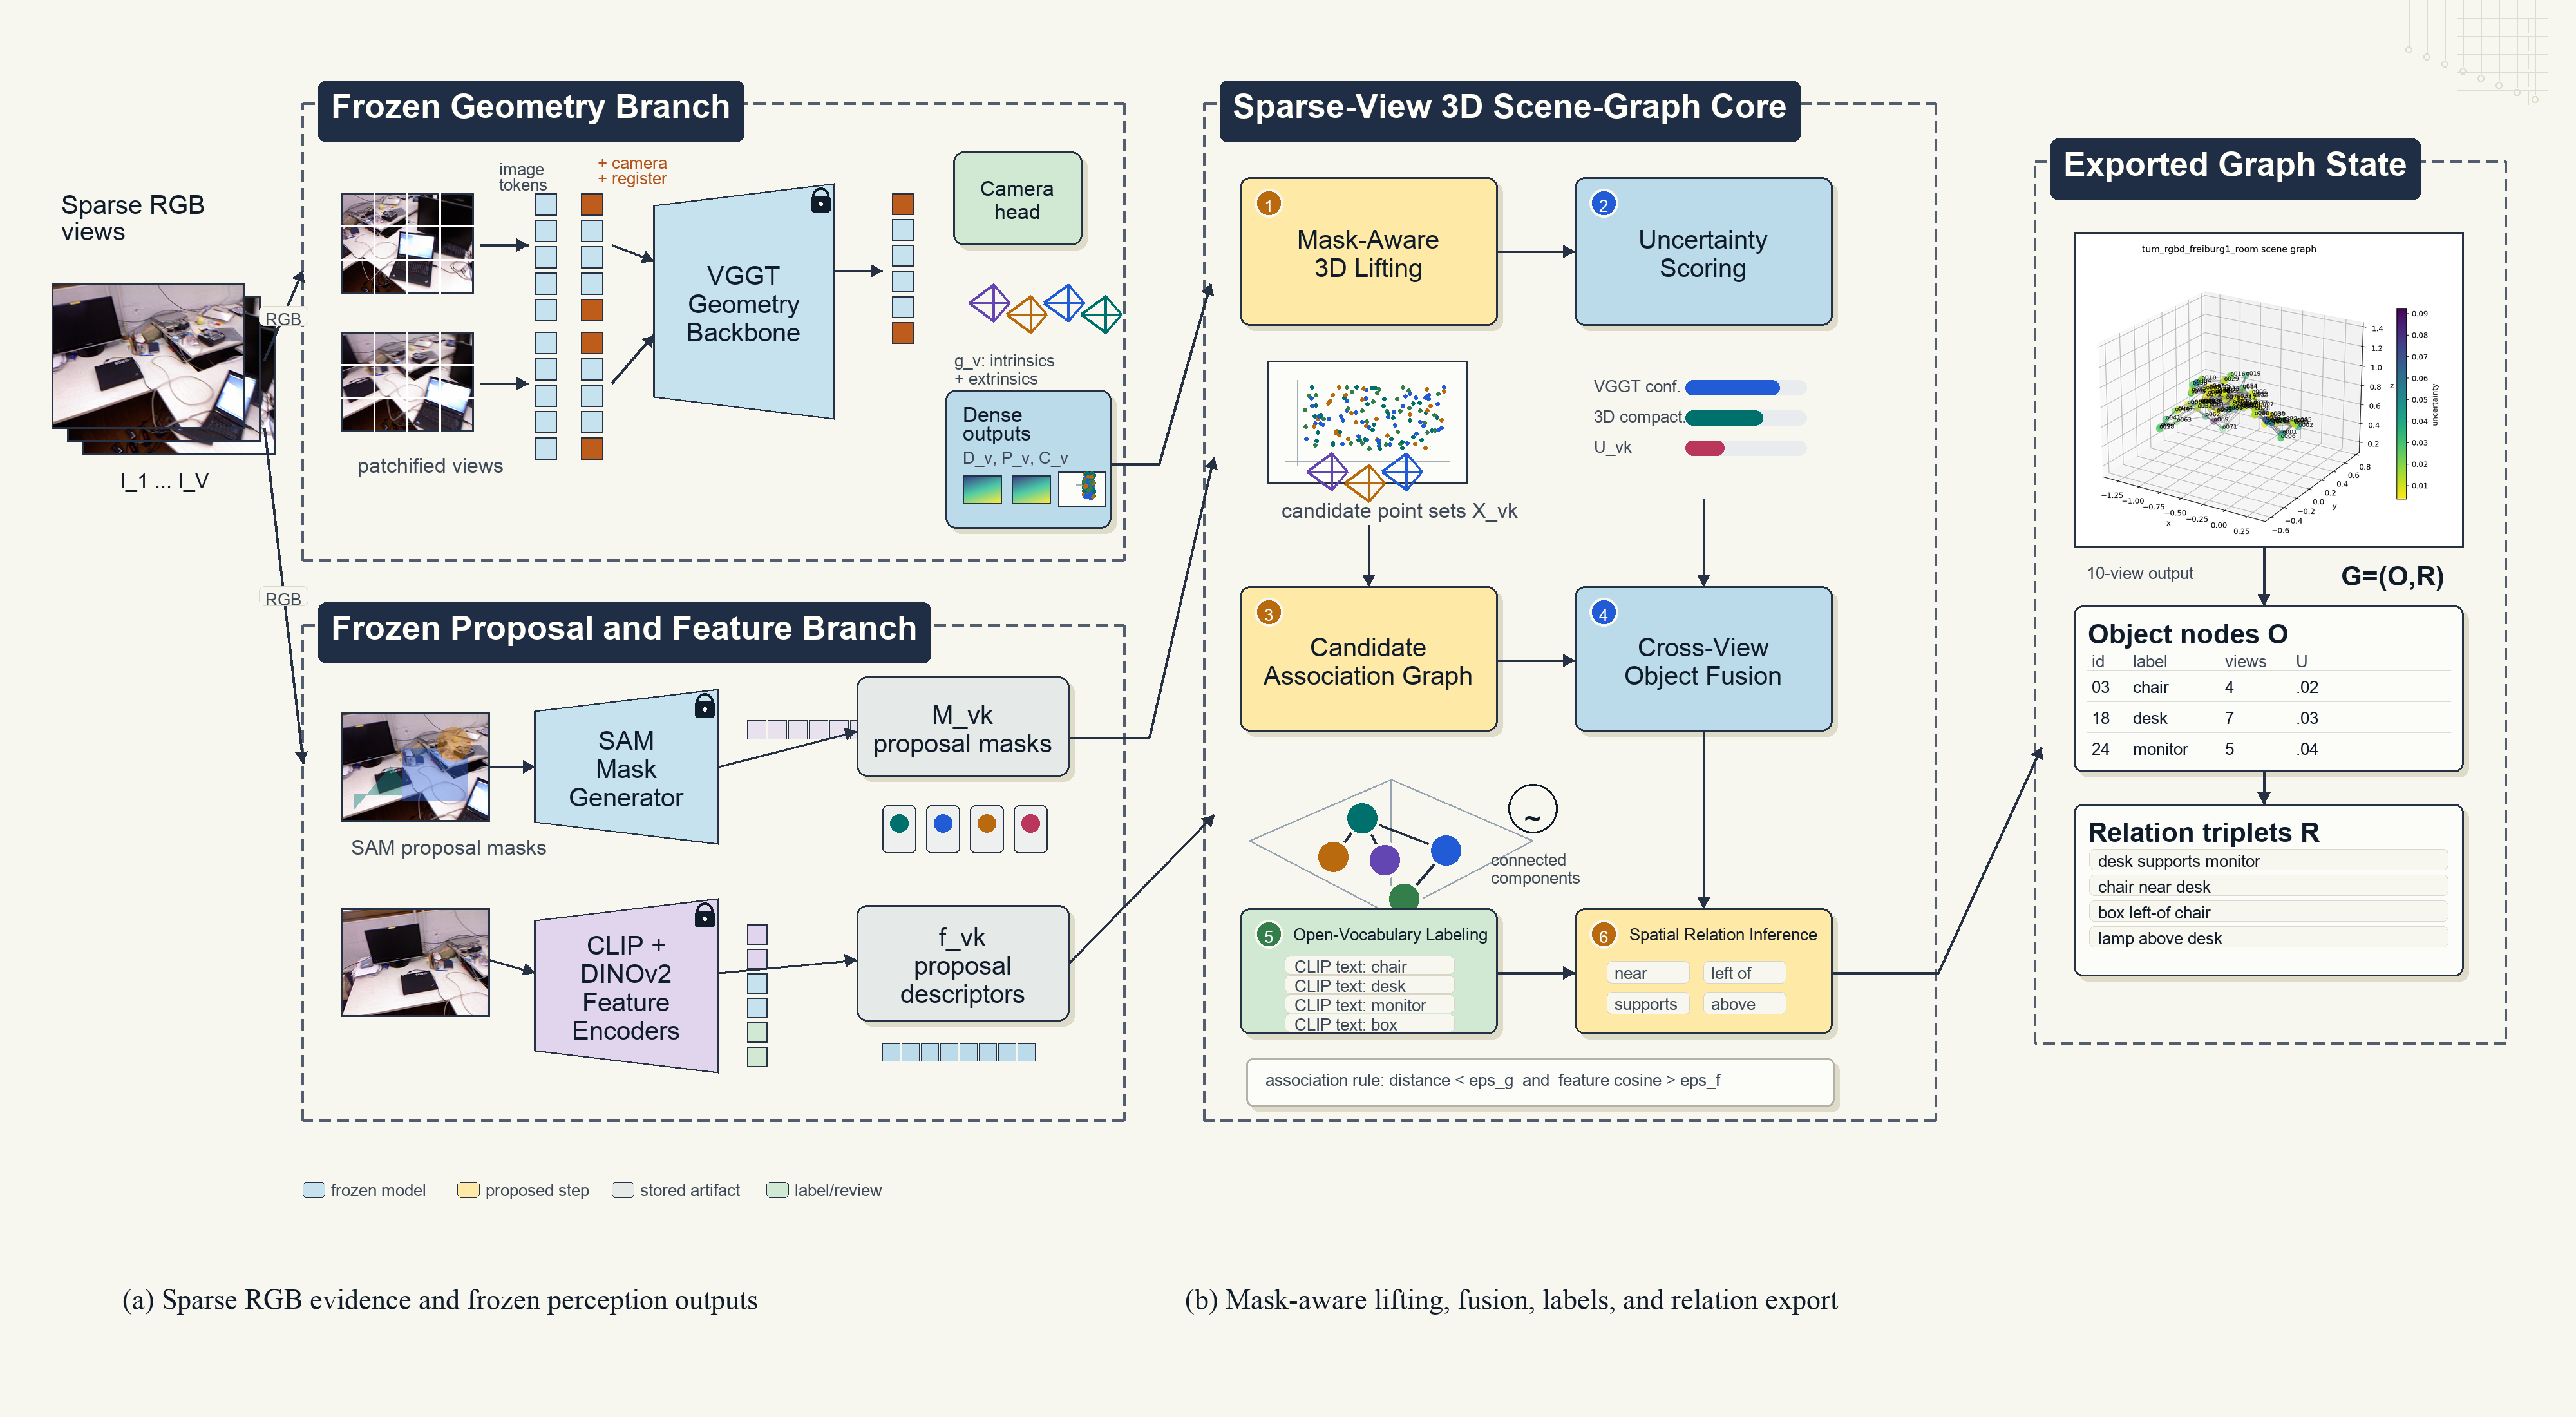
\includegraphics[width=0.98\textwidth]{figures/method_pipeline}
\caption{Architecture of the proposed sparse-view 3D scene graph system. The figure
shows the actual artifacts passed between stages: sparse RGB frames, patch and camera
tokens, frozen VGGT camera/depth/world-point/confidence outputs, SAM masks,
CLIP+DINOv2 proposal descriptors, lifted 3D candidate point sets, uncertainty scores,
association edges, fused objects, open-vocabulary labels, relation predicates, and the
exported scene graph $\mathcal{G}=(\mathcal{O},\mathcal{R})$.}
\label{fig:method_pipeline}
\end{figure}

\subsection{Overview}

The pipeline has five stages. First, VGGT predicts camera parameters, depth maps,
world-point maps, and confidence maps for the selected sparse views. Second, SAM
generates view-local object proposals, and CLIP+DINOv2 descriptors are extracted for
each proposal. Third, every proposal mask is lifted into the VGGT world-point map to
form a 3D candidate object fragment with a confidence and compactness uncertainty
score. Fourth, candidates from different views are connected when they are close in 3D
and sufficiently similar in descriptor space; connected components become fused object
nodes. Fifth, fused nodes are assigned open-vocabulary labels and connected by spatial
relation predicates. The output graph keeps the predicted labels and relations together
with the evidence used to produce them, so the graph can be inspected or converted into
annotation review packets.

\subsection{Sparse-View Geometry}

We run VGGT on the selected sparse views and save camera intrinsics, extrinsics, depth
maps, world-point maps, and confidence maps~\cite{wang2025vggt}. The world-point map
for each view acts as a 2D-to-3D lookup table. This is the key simplification: object
proposals can be lifted directly from image coordinates into a common 3D frame without
first reconstructing a mesh, running bundle adjustment, or optimizing a radiance-field
or Gaussian Splatting representation~\cite{schonberger2016sfm,mildenhall2020nerf,kerbl2023gaussian}.
For view $v$, we denote the world-point map by $P_v(u) \in \mathbb{R}^3$ and the
corresponding confidence map by $C_v(u)$ at image coordinate $u$.

\subsection{2D Proposals and Features}

SAM produces class-agnostic masks for each view~\cite{kirillov2023segment}. For
proposal $k$ in view $v$, we store the bounding box, confidence score, RLE mask, and
visual descriptors. CLIP supplies the language-aligned component, while DINOv2 adds a
complementary self-supervised appearance signal~\cite{radford2021clip,oquab2023dinov2}.
When both descriptors are available, the normalized vectors are concatenated and
renormalized:
\begin{equation}
    f_{v,k} =
    \frac{[\hat{f}^{\mathrm{CLIP}}_{v,k};\hat{f}^{\mathrm{DINO}}_{v,k}]}
    {\|[\hat{f}^{\mathrm{CLIP}}_{v,k};\hat{f}^{\mathrm{DINO}}_{v,k}]\|_2}.
\end{equation}
If one descriptor is unavailable, the valid normalized descriptor is retained. This
keeps the fusion stage usable across proposal files with different feature backends.

\subsection{Mask-Aware 3D Lifting}

Each 2D proposal mask $M_{v,k}$ is resized to the VGGT geometry resolution. The mask
selects world points from the corresponding view, while non-finite points and points
below the confidence threshold $\tau_c$ are discarded:
\begin{equation}
    X_{v,k} = \{P_v(u) \mid u \in M_{v,k},\, C_v(u) \geq \tau_c\}.
\end{equation}
Proposals with no valid lifted points are rejected. The remaining candidate node
stores a sampled 3D point set $X_{v,k}$, centroid $\mu_{v,k}$, 3D bounding box,
proposal metadata, visual feature $f_{v,k}$, and an uncertainty score. The uncertainty
combines VGGT point confidence with the spatial compactness of the lifted 3D points:
\begin{equation}
    U_{v,k} = \lambda(1-\bar{C}_{v,k}) + (1-\lambda)\,
    \mathrm{clip}\left(\frac{\sigma(X_{v,k})}{s_0},0,1\right),
\end{equation}
where $\bar{C}_{v,k}$ is the mean confidence of the selected points and
$\sigma(X_{v,k})$ summarizes spread around the median 3D point. In the implementation,
$\lambda=0.7$ and $s_0=1$. The score is not treated as an oracle; it is exported with
each node and used to prioritize ambiguous objects for later inspection.

\subsection{Graph Fusion}

Candidate nodes are fused by building an association graph over lifted proposals. We
disallow same-view association edges by default, so a component represents cross-view
object support rather than grouping proposals from a single image. An edge connects two
candidates when their centroids are close in 3D and, when valid descriptors exist,
their cosine similarity exceeds a feature threshold:
\begin{equation}
    \|\mu_a-\mu_b\|_2 \leq \epsilon_g
    \quad\mathrm{and}\quad
    \cos(f_a,f_b) \geq \epsilon_f.
\end{equation}
The feature condition is omitted for candidates without valid descriptors. Connected
components define fused object identities. For each component, points are pooled and
sampled, descriptors are averaged and renormalized, and the uncertainty is averaged
then reduced according to the number of supporting views. This separates view-local
evidence from object identity while preserving the proposal provenance needed for
debugging and annotation.

\subsection{Relation Inference and Labeling}

Spatial relations are inferred from fused centroids using distance and relative
coordinate rules. The relation vocabulary includes \emph{near}, \emph{left\_of},
\emph{right\_of}, \emph{above}, \emph{below}, \emph{in\_front\_of}, and
\emph{behind}. A near relation is emitted for object pairs within a distance threshold;
otherwise the vertical displacement or dominant horizontal coordinate determines the
directional predicate, with an optional maximum relation distance limiting very distant
pairs. For language grounding, fused nodes are labeled by comparing averaged visual
descriptors against CLIP text embeddings from an open-vocabulary label
set~\cite{radford2021clip}. The exported graph preserves both symbolic fields and
numeric support data, allowing the same object identities, point sets, labels, and
uncertainty values to be reused by manual review or future learned relation heads.
